\documentclass[11pt,compress,t,notes=noshow, xcolor=table]{beamer}
\usepackage[]{graphicx}\usepackage[]{color}
% maxwidth is the original width if it is less than linewidth
% otherwise use linewidth (to make sure the graphics do not exceed the margin)
\makeatletter
\def\maxwidth{ %
  \ifdim\Gin@nat@width>\linewidth
    \linewidth
  \else
    \Gin@nat@width
  \fi
}
\makeatother

\definecolor{fgcolor}{rgb}{0.345, 0.345, 0.345}
\newcommand{\hlnum}[1]{\textcolor[rgb]{0.686,0.059,0.569}{#1}}%
\newcommand{\hlstr}[1]{\textcolor[rgb]{0.192,0.494,0.8}{#1}}%
\newcommand{\hlcom}[1]{\textcolor[rgb]{0.678,0.584,0.686}{\textit{#1}}}%
\newcommand{\hlopt}[1]{\textcolor[rgb]{0,0,0}{#1}}%
\newcommand{\hlstd}[1]{\textcolor[rgb]{0.345,0.345,0.345}{#1}}%
\newcommand{\hlkwa}[1]{\textcolor[rgb]{0.161,0.373,0.58}{\textbf{#1}}}%
\newcommand{\hlkwb}[1]{\textcolor[rgb]{0.69,0.353,0.396}{#1}}%
\newcommand{\hlkwc}[1]{\textcolor[rgb]{0.333,0.667,0.333}{#1}}%
\newcommand{\hlkwd}[1]{\textcolor[rgb]{0.737,0.353,0.396}{\textbf{#1}}}%
\let\hlipl\hlkwb

\usepackage{framed}
\makeatletter
\newenvironment{kframe}{%
 \def\at@end@of@kframe{}%
 \ifinner\ifhmode%
  \def\at@end@of@kframe{\end{minipage}}%
  \begin{minipage}{\columnwidth}%
 \fi\fi%
 \def\FrameCommand##1{\hskip\@totalleftmargin \hskip-\fboxsep
 \colorbox{shadecolor}{##1}\hskip-\fboxsep
     % There is no \\@totalrightmargin, so:
     \hskip-\linewidth \hskip-\@totalleftmargin \hskip\columnwidth}%
 \MakeFramed {\advance\hsize-\width
   \@totalleftmargin\z@ \linewidth\hsize
   \@setminipage}}%
 {\par\unskip\endMakeFramed%
 \at@end@of@kframe}
\makeatother

\definecolor{shadecolor}{rgb}{.97, .97, .97}
\definecolor{messagecolor}{rgb}{0, 0, 0}
\definecolor{warningcolor}{rgb}{1, 0, 1}
\definecolor{errorcolor}{rgb}{1, 0, 0}
\newenvironment{knitrout}{}{} % an empty environment to be redefined in TeX

\usepackage{alltt}
\newcommand{\SweaveOpts}[1]{}  % do not interfere with LaTeX
\newcommand{\SweaveInput}[1]{} % because they are not real TeX commands
\newcommand{\Sexpr}[1]{}       % will only be parsed by R
\newcommand{\xmark}{\ding{55}}%


\usepackage[english]{babel}
\usepackage[utf8]{inputenc}

\usepackage{dsfont}
\usepackage{verbatim}
\usepackage{amsmath}
\usepackage{amsfonts}
\usepackage{amssymb}
\usepackage{bm}
\usepackage{csquotes}
\usepackage{multirow}
\usepackage{longtable}
\usepackage{booktabs}
\usepackage{enumerate}
\usepackage[absolute,overlay]{textpos}
\usepackage{psfrag}
\usepackage{algorithm}
\usepackage{algpseudocode}
\usepackage{eqnarray}
\usepackage{arydshln}
\usepackage{tabularx}
\usepackage{placeins}
\usepackage{tikz}
\usepackage{setspace}
\usepackage{colortbl}
\usepackage{mathtools}
\usepackage{wrapfig}
\usepackage{bm}
\usepackage{amsmath}
\usepackage{pifont}
\usepackage{xcolor} %colored math symbols

\usetikzlibrary{shapes,arrows,automata,positioning,calc,chains,trees, shadows}
\tikzset{
  %Define standard arrow tip
  >=stealth',
  %Define style for boxes
  punkt/.style={
    rectangle,
    rounded corners,
    draw=black, very thick,
    text width=6.5em,
    minimum height=2em,
    text centered},
  % Define arrow style
  pil/.style={
    ->,
    thick,
    shorten <=2pt,
    shorten >=2pt,}
}

\usepackage{subfig}

% Defines macros and environments
\usepackage{../../style/lmu-lecture}


\let\code=\texttt
\let\proglang=\textsf

\setkeys{Gin}{width=0.9\textwidth}

\setbeamertemplate{frametitle}{\expandafter\uppercase\expandafter\insertframetitle}

\usepackage{bbm}
% basic latex stuff
\newcommand{\pkg}[1]{{\fontseries{b}\selectfont #1}} %fontstyle for R packages
\newcommand{\lz}{\vspace{0.5cm}} %vertical space
\newcommand{\dlz}{\vspace{1cm}} %double vertical space
\newcommand{\oneliner}[1] % Oneliner for important statements
{\begin{block}{}\begin{center}\begin{Large}#1\end{Large}\end{center}\end{block}}


%new environments
\newenvironment{vbframe}  %frame with breaks and verbatim
{
 \begin{frame}[containsverbatim,allowframebreaks]
}
{
\end{frame}
}

\newenvironment{vframe}  %frame with verbatim without breaks (to avoid numbering one slided frames)
{
 \begin{frame}[containsverbatim]
}
{
\end{frame}
}

\newenvironment{blocki}[1]   % itemize block
{
 \begin{block}{#1}\begin{itemize}
}
{
\end{itemize}\end{block}
}

\newenvironment{fragileframe}[2]{  %fragile frame with framebreaks
\begin{frame}[allowframebreaks, fragile, environment = fragileframe]
\frametitle{#1}
#2}
{\end{frame}}


\newcommand{\myframe}[2]{  %short for frame with framebreaks
\begin{frame}[allowframebreaks]
\frametitle{#1}
#2
\end{frame}}

\newcommand{\remark}[1]{
  \textbf{Remark:} #1
}


\newenvironment{deleteframe}
{
\begingroup
\usebackgroundtemplate{
\includegraphics[width=\paperwidth,height=\paperheight]{../style/color/red.png}}
 \begin{frame}
}
{
\end{frame}
\endgroup
}
\newenvironment{simplifyframe}
{
\begingroup
\usebackgroundtemplate{
\includegraphics[width=\paperwidth,height=\paperheight]{../style/color/yellow.png}}
 \begin{frame}
}
{
\end{frame}
\endgroup
}\newenvironment{draftframe}
{
\begingroup
\usebackgroundtemplate{
\includegraphics[width=\paperwidth,height=\paperheight]{../style/color/green.jpg}}
 \begin{frame}
}
{
\end{frame}
\endgroup
}
% https://tex.stackexchange.com/a/261480: textcolor that works in mathmode
\makeatletter
\renewcommand*{\@textcolor}[3]{%
  \protect\leavevmode
  \begingroup
    \color#1{#2}#3%
  \endgroup
}
\makeatother


\input{../../latex-math/basic-math}
\input{../../latex-math/basic-ml}
\input{../../latex-math/ml-nn}

\title{Deep Learning}

\date{}

\begin{document}
\newcommand{\titlefigure}{plots/perturbation.png}
%modify picture
\newcommand{\learninggoals}{
  \item Basics of adversarial training 
  \item Adversarial training for linear models
  %\item Principal component analysis
}

\lecturechapter{Adversarial Training Basics}
\lecture{I2DL}


\newcommand{\Dsubtrain}{\mathcal{D}_{\text{subtrain}}}
\newcommand{\Dval}{\mathcal{D}_{\text{val}}}

% % %%%%%%%%%%%%%%%%%%%%%%%%%%%%%%%%%%%%%%%%%%%%%%%%%%%%%%%%%%%%%%%%%%
% 
% \begin{frame}{Adversarial Robustness}
%     \begin{itemize}
%         \item It is critical to examine if a trained neural net is robust and reliable. 
%         \item \textbf{Adversarial robustness} of a model means that a model is robust to (test time) perturbations of its inputs. 
%         \item \textbf{Adversarial machine learning} studies techniques which attempt  to fool machine learning models through malicious input.
%         \item To make a model more robust, we can train our model on adversarially perturbed examples, called \textbf{adversarial examples}, derived from the training set.  
%         \item This chapter summarizes  high-level ideas in adversarial robustness with a particular emphasis on adversarial examples.
%         \item For a deeper dive, \href{https://adversarial-ml-tutorial.org/}{\beamergotobutton{click here.}}
%     \end{itemize}
% \end{frame}
% 
% 
% %%%%%%%%%%%%%%%%%%%%%%%%%%%%%%%%%%%%%%%%%%%%%%%%%%%%%%%%%%%%%%%%%%
% \section{Adversarial Examples}
% %%%%%%%%%%%%%%%%%%%%%%%%%%%%%%%%%%%%%%%%%%%%%%%%%%%%%%%%%%%%%%%%%%
% 
%  \begin{frame} {Adversarial Examples}
%    \begin{itemize}
%      \item An adversarial example is an input to a model that is deliberately designed to "fool" the model into misclassifying it.
%      \item The test error of a model is only an indicator of how well the model performs with respect to samples from the data-generating distribution.
%      \item The performance of the same model can be drastically different on samples from a completely different distribution (on the same input space).
%       \item It is possible to make changes to an image that makes a pretrained CNN (for example) output a completely different predicted class even though the change is imperceptible to the human eye.
%      \item These examples suggest that even models that have very good test set performance do not have a deep understanding of the underlying concepts that determine the correct output label.
%      \end{itemize}
%     \end{frame}
%     
%   \begin{frame} {Adversarial Examples}
%     \begin{itemize}
%       \item Adversarial examples are \textit{not} unique to deep neural nets. Many other models (such as logistic regression) are also susceptible to them.
%       \item They pose serious security concerns in many areas.
%       \item Example: Fooling autonomous cars into thinking that a stop sign is a 45 km/h sign.
%       \item Example: Evading law enforcement by fooling facial recognition systems into misidentifying individuals.
%    \end{itemize}
%  \end{frame}
%  
%  \begin{frame} {Adversarial Examples}
%   \begin{figure}
%     \centering
%        \captionsetup{font=footnotesize,labelfont=footnotesize, labelfont = bf}
%       \scalebox{1}{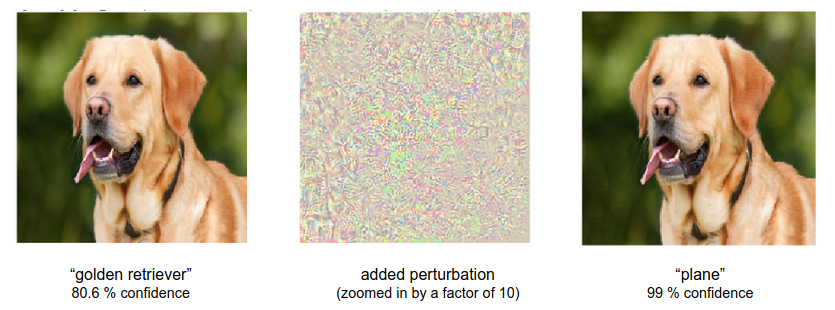
\includegraphics{plots/dog.png}}
%       \tiny{\\Credit: Maxence Prevost}
%       \caption{\footnotesize The difference between the left and the right golden retriever is imperceptible to humans.
%       The last image was classified as a plane by ResNet50 with more than 99\% confidence. 
%       The only difference between the left and right image are small pixel perturbations, shown in the second picture.}
%   \end{figure}
% \end{frame}
% 
% \begin{frame} {Adversarial Examples}
%   \begin{figure}
%     \centering
%        \captionsetup{font=footnotesize,labelfont=footnotesize, labelfont = bf}
%       \scalebox{1}{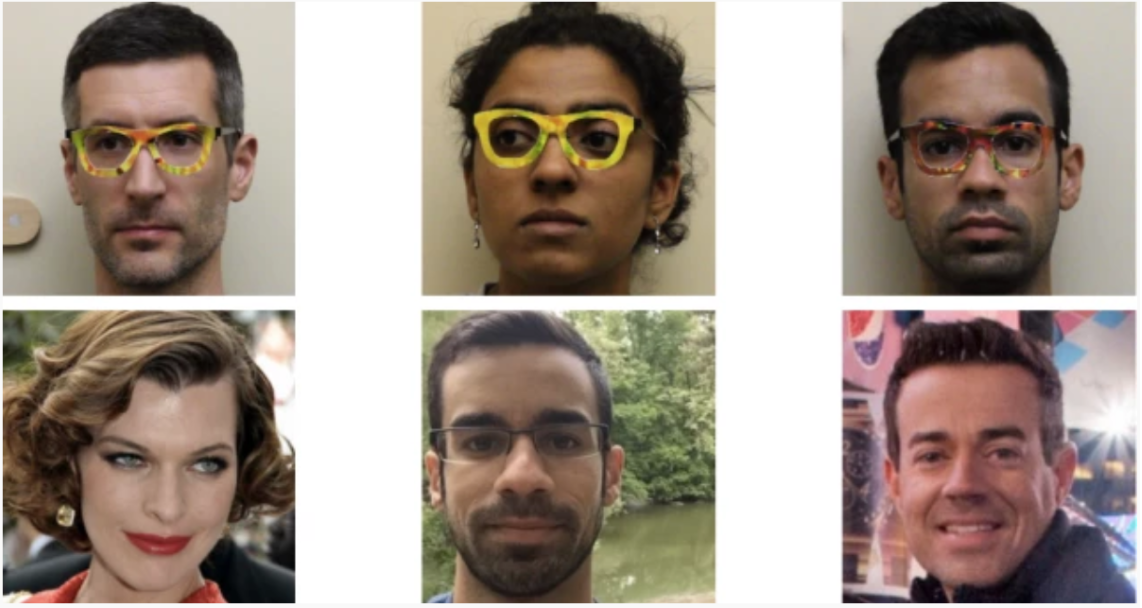
\includegraphics{plots/glasses.png}}
%       \tiny{\\Credit: Sharif et al.}
%       \caption{\footnotesize A CNN misidentified each person in the top row (with the funky looking "adversarial" glasses) as the one in the corresponding position in the bottom row. The generated images do often contain some features of the target class.}
%   \end{figure}
% \end{frame}
% 
% \begin{frame} {Adversarial Examples}
%   \begin{figure}
%     \centering
%        \captionsetup{font=footnotesize,labelfont=footnotesize, labelfont = bf}
%       \scalebox{0.8}{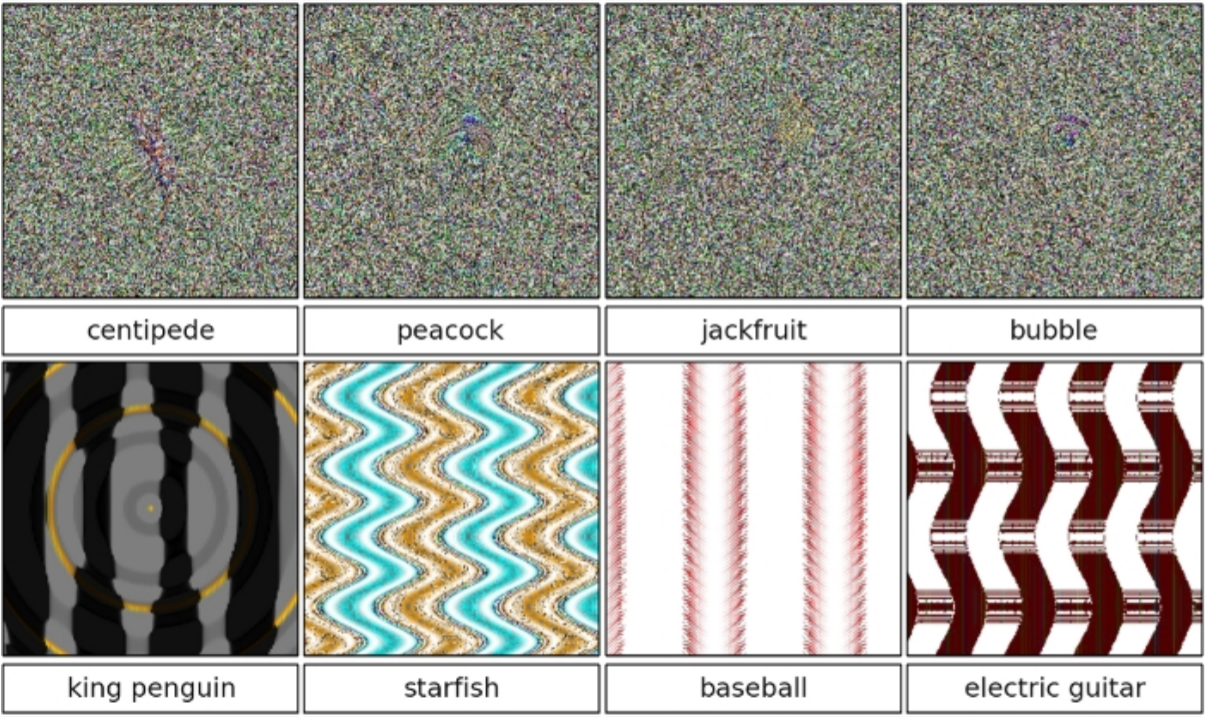
\includegraphics{plots/easyfooled.png}}
%       \tiny{\\Credit: Nguyen et al.}
%       \caption{\footnotesize All 8 images above are unrecognizable to humans but are misclassified by a CNN with higher than 99\% confidence.  The CNN was trained by Krizhevsky et al. on the ImageNet dataset and consists of five convolutional layers, some of which are followed by max-pooling layers,and three fully-connected layers with a final softmax.}
%   \end{figure}
% \end{frame}
% 
% \begin{frame} {Adversarial Examples}
%   \begin{figure}
%     \centering
%       \scalebox{0.8}{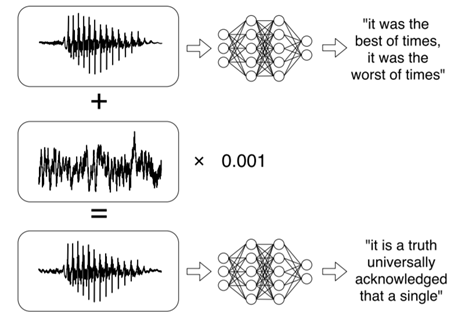
\includegraphics{plots/adv_speech.png}}
%       \tiny{\\Credit: Carlini et al}
%       \caption{\footnotesize  It is possible to add a small perturbation to any waveform in order to fool a speech-to-text neural network into transcribing it as any desired target phrase. 
%       %(This was not generated using FGSM.)
%       }
%   \end{figure}
% \end{frame}
% 
% %%%%%%%%%%%%%%%%%%%%%%%%%%%%%%%%%%%%%%%%%%%%%%%%%%%%%%%%%%%%%%%%%%
% %\section{Creation of Adversarial Examples}
% %%%%%%%%%%%%%%%%%%%%%%%%%%%%%%%%%%%%%%%%%%%%%%%%%%%%%%%%%%%%%%%%%%
% \begin{vbframe} {Creation of Adversarial Examples}
%   \begin{itemize}
%   \item In the examples earlier, we saw that adversarial examples can seem recognizable to humans or seem like random noise/patterns.
%   \item In the following, given a datapoint $\xv$, we want to create an adversarial example $\tilde{\xv}$ that is very similar to $\xv$. 
%     %\item The Fast Gradient Sign Method (FGSM) is a very simple way to generate adversarial examples.
%     \item Specifically, our goal is to find an input $\tilde{\xv}$ close to the datapoint $\xv$ such that a pretrained model (which accurately classifies $\xv$), ends up misclassifying $\tilde{\xv}$. 
%     % even though $\tilde{\xv}$ is visually indistinguishable from $\xv$ to human beings.
%     \item When we train a neural network, we typically want to optimize the parameter $\thetab$, so that we minimize the loss. 
%     \item By contrast, to find an adversarial example $\tilde{\xv}$ that is in the vicinity of $\xv$, we want to optimize the \textit{input} to \textit{maximize} the loss.    \framebreak
%     \item To ensure that $\tilde{\xv}$ is close to $\xv$, we optimize over the perturbation of $\xv$, denoted as $\deltab$, and define an feasible set of perturbations $\Delta$. 
%     \begin{equation*}
%         \argmax_{\deltab \in \Delta} L(y, \fh(\xv + \deltab| \thetab))
%     \end{equation*}
%     \item A common perturbation set is $\mathcal{B}^{\infty}_{\epsilon}$ which is the $\epsilon$-ball measured by $\ell_{\infty} = \|\cdot\|_{\infty}$
%     \begin{equation*}
%         \Delta = \mathcal{B}^{\infty}_{\epsilon}(\deltab) = \{\deltab: ||\deltab||_{\infty} \le \epsilon\} \text{ with } ||\deltab||_{\infty} = \max_i|\delta_i|
%     \end{equation*}
%     It allows each component of the perturbation $\deltab$ to lie between  $-\epsilon$ and $+ \epsilon$.
%     \item In general, $\Delta$ can also depend on the input datapoint $\xv$, denoted as $\Delta(\xv)$.
%   \end{itemize}
% \end{vbframe}
% 
% \begin{frame} {Example: ResNet50}
%   \begin{figure}
%     \centering
%       \scalebox{1}{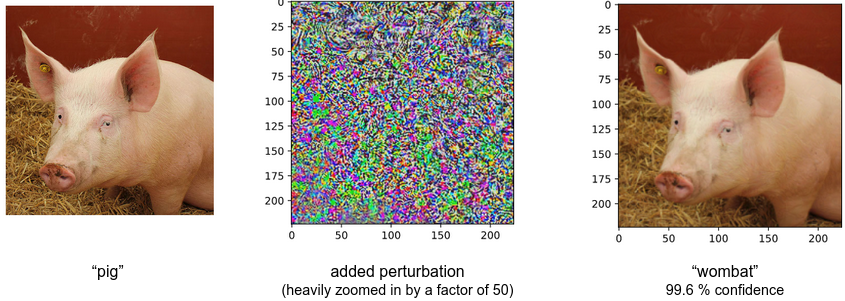
\includegraphics{plots/pig.png}}
%      \tiny{\\Credit: Kolter \& Madry}
%      \vspace{-0.2cm}
%       \caption{Adversarial example for one datapoint of the ImageNet dataset and pre-trained ResNet50. By adding an imperceptibly small perturbation to the original image,  an image was created that looks identical to our original image, but is misclassified.}
%   \end{figure}
% \end{frame}
% 
% \begin{frame}{Targeted Attacks}
%     \begin{itemize}
%         \item It is also possible to generate adversarial examples classified virtually as any desired class. This is known as a \textbf{targeted attack}.
%         \item The only difference is that, instead of trying to just maximize the loss of the correct class, we maximize the loss of the correct class while also minimizing the loss of a target class $y_{target}$.
%         \begin{equation*}
%              \argmax_{\deltab \in \Delta} ( L(y, \fh(\xv + \deltab| \thetab)) - L(y_{target}, \fh(\xv + \deltab| \thetab)) )
%         \end{equation*}
%     \end{itemize}
% \end{frame}
% % \begin{frame} {Other forms}
% % In practice, adversarial examples of images can be generated not only by making small modifications to the input pixels, but also using spatial transformations.
% %         \begin{figure}
% %    \captionsetup{font=footnotesize,labelfont=footnotesize, labelfont = bf}
% %     \centering
% %       \scalebox{0.6}{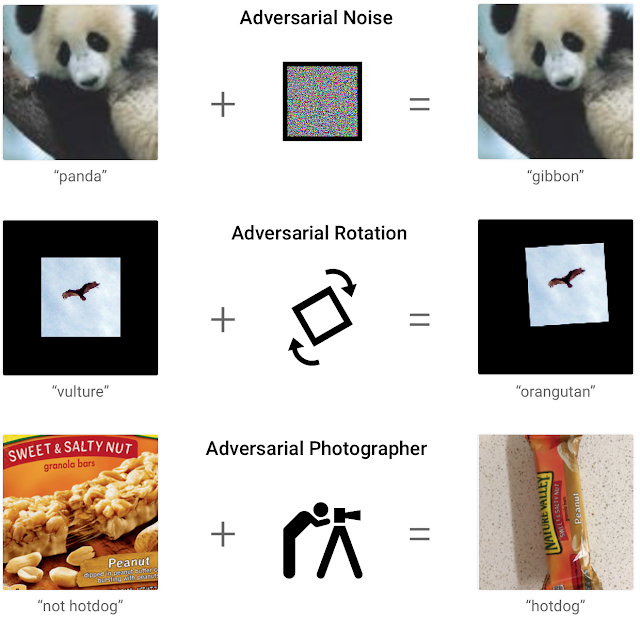
\includegraphics{plots/adversarials_forms.png}}
% %      \tiny{\\Credit: Brown (2018)}
% %   \end{figure}
% % \end{frame}
%   
% %%%%%%%%%%%%%%%%%%%%%%%%%%%%%%%%%%%%%%%%%%%%%%%%%%%%%%%%%%%%%%%%%%
% \section{Adversarial  Training}
%%%%%%%%%%%%%%%%%%%%%%%%%%%%%%%%%%%%%%%%%%%%%%%%%%%%%%%%%%%%%%%%%%
\begin{vbframe}{Adversarial Training}
    \begin{itemize}
        \item To modify a trained model so that it is more resistant to such attacks, adversarial training can be performed. 
        \lz
%        \item Adversarial training can be seen as a form of regularization.
          \lz
        \item To do so, we minimize the \textbf{empirical adversarial risk} which measures the worst-case empirical loss of a model, if we are able to manipulate every input $\xv$ in the training data set within the feasible set $\Delta(\xv)$:
        \begin{equation*}
            \min_{\thetab} \risk_{adv}(\thetab) = \min_{\thetab} \frac{1}{N} \sum_{i = 1}^{N} \max_{\deltab \in \Delta(\xv)} \Lossdeltai
        \end{equation*}
          
          \framebreak
      
        \item To solve the optimization problem, we use SGD over $\thetab$. In each SGD step $t \in \{1, 2,...\}$ we repeatedly choose a minibatch of size $m$ and repeat the following until a stopping criterion is met: 
        \begin{enumerate}
            \item For each $(\xi, \yi), i = 1, ..., m$, we compute an adversarial example 
            \begin{equation*}
                \deltab^{*}(\xi) = \argmax_{\deltab \in \Delta(\xi)} L(\yi, f(\xi + \deltab| \thetab^{[t]}))
            \end{equation*}
            \item Then we compute the gradient of the empirical adversarial risk given $\deltab^* = (\deltab^*(\xv^{(1)}), ..., \deltab^*(\xv^{(m)}))$ and update $\thetab$: 
            \begin{equation*}
                \thetab^{[t+1]} := \thetab^{[t]} - \alpha \frac{1}{m} \sum_{i = 1}^{m} \nabla_{\thetab} L(\yi, f(\xi + \deltab^*(\xi)| \thetab^{[t]}))
            \end{equation*}
        \end{enumerate}
        \item The first step is derived from Danskin's theorem, which states that the gradient of the inner function (maximization term) is simply given by the gradient of the function evaluated at its maximum.
    \end{itemize}
\end{vbframe}

%%%%%%%%%%%%%%%%%%%%%%%%%%%%%%%%%%%%%%%%%%%%%%%%%%%%%%%%%%%%%%%%%%
\section{Linear Models}
%%%%%%%%%%%%%%%%%%%%%%%%%%%%%%%%%%%%%%%%%%%%%%%%%%%%%%%%%%%%%%%%%%
\begin{vbframe} {Linear Models}
  \begin{itemize}
    \item In case of linear models, the inner maximization problem can be solved exactly. We show this in the case of binary classification using linear models.
    \item Recall, the hypothesis space for logistic regression consists of models of the form:
          \small
          $$\Hspace = \left\{f: \mathbb{R}^p \to [0, 1] ~\bigg|~ \fx = \tau\left(\sum_{j = 1}^p \theta_j x_j + \theta_0 \right), \thetab \in \mathbb{R}^p, \theta_0 \in \mathbb{R} \right\},$$
          \normalsize
          where $\tau(z) = (1 + \exp(-z))^{-1}$ is the logistic sigmoid function. 
    \item For class labels $y \in \{+1,-1\}$ , the logistic loss is:
          \small
          $$\Lxyt = \log(1 + \exp(- {y (\underbrace{\sum_{j = 1}^p \theta_j x_j}_{\thetab^T\xv} + \theta_0))}) \equiv \Psi(y (\thetab^T\xv + \theta_0))$$
          \normalsize
          where we define $\Psi(z) = \log(1+\exp(-z))$.
  \end{itemize}

\framebreak

  \begin{itemize}
    \item The inner maximization in the adversarial risk, which we saw earlier, can be written as:
    $$\max_{\deltab \in \Delta(\xv)} \Lossdelta = \max_{\deltab \in \Delta(\xv)} \Psi(y (\thetab^T(\xv + \deltab) + \theta_0)) $$
    \item In this particular case, it is possible to solve the inner maximization exactly.
    \item First, note that $\Psi$ is a monotonically decreasing function:
    \begin{figure}
    \centering
      \scalebox{0.5}{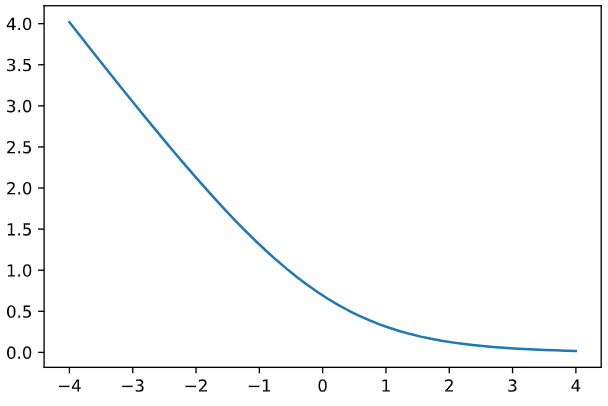
\includegraphics{plots/logistic_loss.png}}
      \tiny{\\Kolter \& Madry, 2019}
    \end{figure}
  \end{itemize}

\framebreak

  \begin{itemize}
    \item Maximizing such a monotonically decreasing function is equivalent to minimizing the argument.
    \lz
    \item Therefore
          \begin{align*}
            \max_{\deltab \in \Delta(\xv)} \Psi(y (\thetab^T(\xv + \deltab) + \theta_0)) &= \Psi(\min_{\deltab \in \Delta(\xv)}y (\thetab^T(\xv + \deltab) + \theta_0)) \\
                                                                                    &= \Psi (y (\thetab^T\xv + \theta_0) + \min_{\deltab \in \Delta(\xv)} y (\thetab^T \deltab))
          \end{align*}
    \lz
    \item We have to solve the problem
    $$ \min_{\deltab \in \Delta} y (\thetab^T \deltab) $$
  \end{itemize}

\framebreak

  \begin{itemize}
    \item To get a feel for the problem, let us consider the case where $y = +1$ and use $\Delta = \mathcal{B}^{\infty}_{\epsilon}$. The latter constrains each element of $\delta$ to lie between $-\epsilon$ and $+\epsilon$.
    \lz
    \item The quantity $y (\thetab^T \deltab)$ is then minimized when $\delta_j = - \epsilon$ for $\theta_{j} \geq 0$ and $\delta_j = \epsilon$ for $\theta_{j}<0$.
    \lz
    \item For $y = -1$, the signs would be flipped.
    \lz
    \item The optimal solution then, is
    $$\deltab^* = -y\epsilon \cdot \sign(\thetab) $$
    \item Note that the optimal solution does not explicitly depend on $\xv$. 

\framebreak

  \item The function value achieved by the solution is: 
  $$y \cdot \thetab^T \deltab^* = y \cdot \sum_j -y \epsilon \cdot \sign(\theta_j)\theta_j = - y^2 \epsilon \sum_j | \theta_j | = -\epsilon\|\thetab\|_{1} $$
  \item Therefore, we have analytically computed the solution to the inner maximization problem! The solution is:
  $$ \max_{\deltab \in \Delta(\xv)} \Psi(y (\thetab^T(\xv + \deltab) + \theta_0)) =  \Psi (y (\thetab^T(\xv + \deltab)) -\epsilon\|\thetab\|_{1}) $$
  \item As a result, the adversarial risk, which was a min-max problem, has now been converted to a pure minimization problem:
  $$\min_{\thetab, \theta_0} \frac{1}{N} \sum_{i = 1}^{N} \Psi \left(\yi \cdot\left(\thetab^{T} \xi +\theta_0\right)-\epsilon\|\thetab\|_{1}\right)$$
  \item This problem is convex in $\{\thetab, \theta_0\}$ and can be solved exactly. An iterative optimizer such as SGD will also approach the global minimum.
  \end{itemize}
  
\end{vbframe}

\begin{vbframe} {MNIST example}

  \begin{itemize}
    \item As an example, we look at the MNIST dataset, but this time we perform logistic regression and focus only on the classification of 0s vs.    1s.
    \lz
    \item The logistic regression classifier was trained for 10 epochs with SGD on the training set. 
    \lz
    \item This model obtained a low misclassification rate of 0.0004 on the test set.  
    \lz
    \item To generate adversarial examples, $\Delta$ is defined as $\mathcal{B}^{\infty}_{0.2}$.
    \lz
    \item As we saw earlier, the optimal perturbation $\deltab^*$ is $-y\epsilon \cdot \sign(\thetab)$.
  \framebreak
  \item As $\deltab^*$ does not directly depend on $\xv$, it is the "same" (ignoring the value of label $y$) across all examples. This is what it looks like:
    \begin{figure}
    \captionsetup{font=footnotesize,labelfont=footnotesize, labelfont = bf}
    \centering
      \scalebox{0.23}{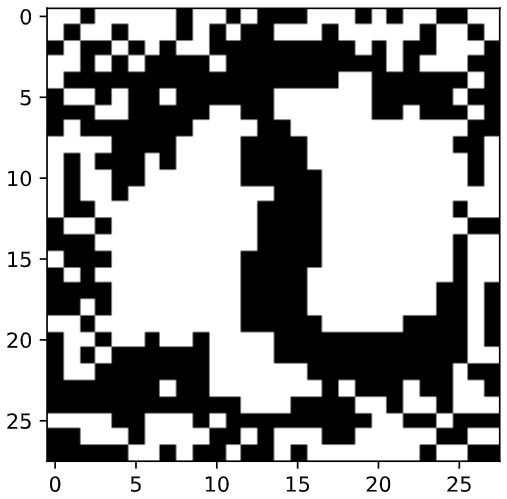
\includegraphics{plots/perturbation.png}}
      %\tiny{\\Credit: Kolter and Madry}
      \caption{The optimal perturbation for images that contain 0. For images that contain 1, the signs would be flipped (Kolter \& Madry, 2019). (The contrast between the black and white pixels is amplified for the sake of visualization.) }
    \end{figure}
    \item The perturbation (\textit{vaguely}) has a vertical line (like a 1) in black pixels, and a circle (like a 0) in white pixels. Intuition: When a given image is moved (translated) in the black direction, it is more likely to be classified as 1, whereas when moved in the white direction, it is more likely to be classified as 0.
 
    \framebreak
    
    \begin{figure}
    \centering
    \captionsetup{font=footnotesize,labelfont=footnotesize, labelfont = bf}
      \scalebox{0.6}{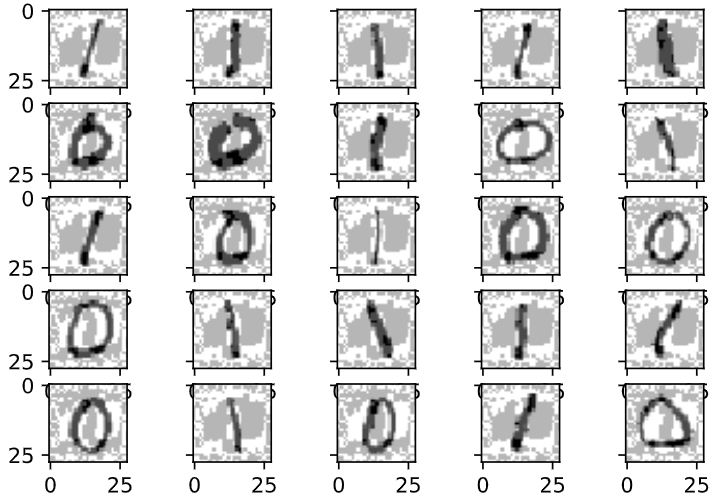
\includegraphics{plots/perturbed.png}}
      %\tiny{\\Credit: Kolter and Madry}
      \caption{Perturbed images from the test set (Kolter \& Madry, 2019).}
    \end{figure}
    
      \item \small{When all the images in test set are perturbed, the misclassification error of the model jumps from 0.0004 to 0.845!
      \item Interestingly, when the model is trained on similarly perturbed images from the training set (that is, the empirical adversarial risk is minimized), the misclassification error on the perturbed test set drops to 0.025.}
    \end{itemize}
    \framebreak
  
  % \begin{itemize}
  %   \item Robust training
  % \end{itemize}
  % 
  % \framebreak
  
    % \begin{figure}
    % \captionsetup{font=footnotesize,labelfont=footnotesize, labelfont = bf}
    % \centering
    %   \scalebox{0.8}{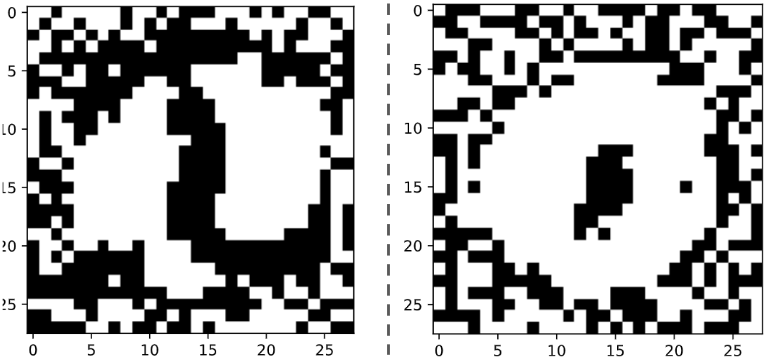
\includegraphics{plots/rob_perturbation.png}}
    %   \tiny{\\source: https://adversarial-ml-tutorial.org/}
    %   \caption{???}
    % \end{figure}
  
\end{vbframe}

% %%%%%%%%%%%%%%%%%%%%%%%%%%%%%%%%%%%%%%%%%%%%%%%%%%%%%%%%%%%%%%%%%%
% \section{Neural Networks}
% %%%%%%%%%%%%%%%%%%%%%%%%%%%%%%%%%%%%%%%%%%%%%%%%%%%%%%%%%%%%%%%%%%
% 
% 
% 
%  \begin{vbframe}{Projected Gradient Descent}
%     \begin{itemize}
%        \item In contrast to logistic regression, neural networks can have a bumpier, 
%        non-convex loss surface.     
%        \item As a consequence, Danskin's theorem does not longer hold and the inner optimization problem must be solved approximately. 
%        \item One approximation method is projected gradient descent (PGD)$^1$.
%         \item Let $\fh$ be the pretrained model, $\xv$ the input to the model, $y$ the target and $L\left(y, \fh(\xv | \thetab) \right)$ the loss function used to train the network.
%         \item In each gradient descent step, the basic PGD algorithm updates $\deltab$ as: 
%         \begin{equation*}
%             \deltab^{[t+1]} = \mathcal{P}\left(\deltab^{[t]} + \alpha \nabla_{\deltab} L\left(y, \fh(\xv + \deltab^{[t]}| \thetab) \right) \right)
%         \end{equation*}
%         where $\mathcal{P}$ denotes the projection onto the ball of interest. \\
%         \lz
%         {\scriptsize $^1$ Technically speaking, it is gradient \textit{ascent} since we are maximizing a function, but for the sake of generality, we just refer to the process here as gradient descent.}
% 
% 
%         %%%%%%%%%%%%%% Original %%%%%%%%%%%%%%%%%%%5
%         % \item In essence, we move with a step size $\alpha$ \textbf{in the direction} of the gradient of the loss with respect to $\deltab$. Then we clip the corresponding values of $\deltab$ back to the chosen perturbation set.  
%         % \item In case of $\Delta$ being $\mathcal{B}^{\infty}_{\epsilon}$ the projection is
%         % \begin{equation*}
%         %     \mathcal{P}_{\Delta}(\deltab) = clip(\deltab, [-\epsilon, \epsilon])
%         % \end{equation*}
%         % \item One gradient step is then defined as 
%         % \begin{equation*}
%         %     \deltab^{[t+1]} = clip\left(\delta^{[t]}+ \alpha \nabla_{\deltab} L\left(y, \fh(\xv | \thetab) \right), [-\epsilon, \epsilon]\right)
%         % \end{equation*}
%         %%%%%%%%%%%%%%%%%%%%%%%%%%%%%%%%%%%%%%%%%%%%%%
%         
%         
%         
%         \item In essence, $\deltab^{[t+1]}$ is obtained by moving from $\deltab^{[t]}$ (with a step size $\alpha$) \textbf{in the direction} of the gradient of the loss with respect to $\deltab$ (evaluated at $\deltab^{[t]}$) and then projecting back to $\Delta$.
%         \item In case where the feasible set is $\mathcal{B}^{\infty}_{\epsilon}$, the projection of an arbitrary vector $\hidz$ is simply:
%         \begin{equation*}
%             \mathcal{P}(\hidz) = clip(\hidz, [-\epsilon, \epsilon])
%         \end{equation*}
%         \item Therefore, when $\Delta$ is $\mathcal{B}^{\infty}_{\epsilon}$, one gradient step is then defined as: 
%         \begin{equation*}
%             \deltab^{[t+1]} = clip\left(\deltab^{[t]}+ \alpha \nabla_{\deltab} L\left(y, \fh(\xv + \deltab^{[t]}| \thetab) \right), [-\epsilon, \epsilon]\right)
%         \end{equation*}
%         \end{itemize}
%         \vspace{-0.5cm}
%           \begin{figure}
%     \centering
%       %\captionsetup{font=footnotesize,labelfont=footnotesize, labelfont = bf}
%       \scalebox{0.85}{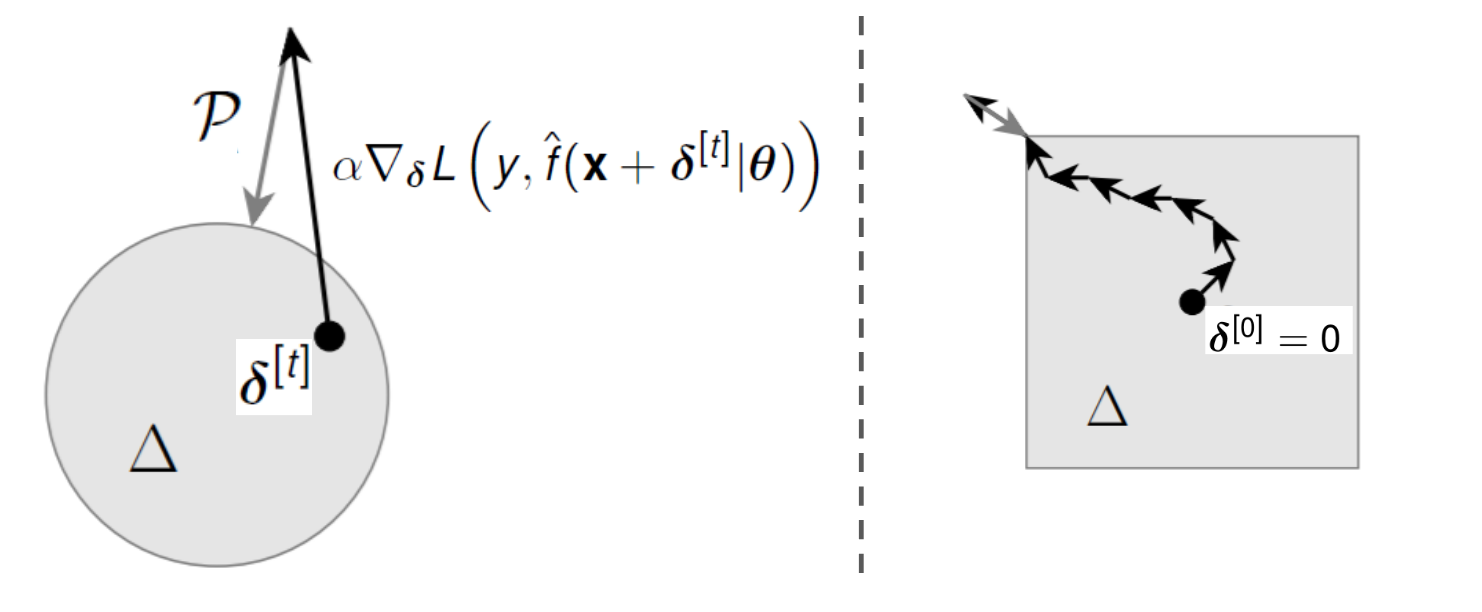
\includegraphics{plots/pgd_mod.png}}
%       \tiny{\\Credit: Kolter and Madry}
%       \caption{\small{\textit{Left}: $\deltab^{[t]}+ \alpha \nabla_{\deltab} L(y, \fh(\xv + \deltab^{[t]}| \thetab))$ is projected back to the perturbation set $\Delta$ using $\mathcal{P}$. Here, $\Delta$ is $\mathcal{B}^{2}_{\epsilon}$.
%       \textit{Right}: Multiple steps of PGD are shown in case of $\Delta = \mathcal{B}^{\infty}_{\epsilon}$; the projection must be only executed in the last step. (Note: A variant of PGD known as \textit{normalized} PGD is shown here. This is why each step has the same size. See Kolter et al. (2019) for details.)}}
%   \end{figure}
%     
% \end{vbframe}
%    
%      \begin{vbframe} {Fast Gradient Sign Method}
%    \begin{itemize}
%    \item Fast Gradient Sign Method (FGSM) is a special case of PGD when $\Delta$ = $\mathcal{B}^{\infty}_{\epsilon}$ and $\alpha \rightarrow \infty$ . 
%    \item As before, the projection of an arbitrary vector $\hidz$ onto $\mathcal{B}^{\infty}_{\epsilon}$ is $\mathcal{P}(\hidz) = clip(\hidz, [-\epsilon, \epsilon])$. 
%    \item As $\alpha \rightarrow \infty$, the elements of $\deltab$ are either set to $-\epsilon$ or $\epsilon$ depending on the sign of the corresponding component of the gradient.
%    \item Thus, the FGSM algorithm computes $\deltab$ as
%    \small
%     \begin{equation*}
%       \deltab = \epsilon sign\left(\nabla_{\xv} L\left(y, \fh(\xv | \thetab) \right) \right)
%     \end{equation*}
%     \normalsize
%     \item Note that for FGSM we only conduct one calculation and not multiple gradient descent steps.
%     \item Furthermore, because we usually initialize $\deltab^{[0]}$ as $0$     
%     \small
%     $$\nabla_{\deltab} L\left(y, \fh(\xv + \deltab | \thetab) \right)  = \nabla_{\xv} L\left(y, \fh(\xv | \thetab) \right)$$
%     \normalsize
%   \begin{figure}
%     \centering
%       \captionsetup{font=footnotesize,labelfont=footnotesize, labelfont = bf}
%       \scalebox{0.32}{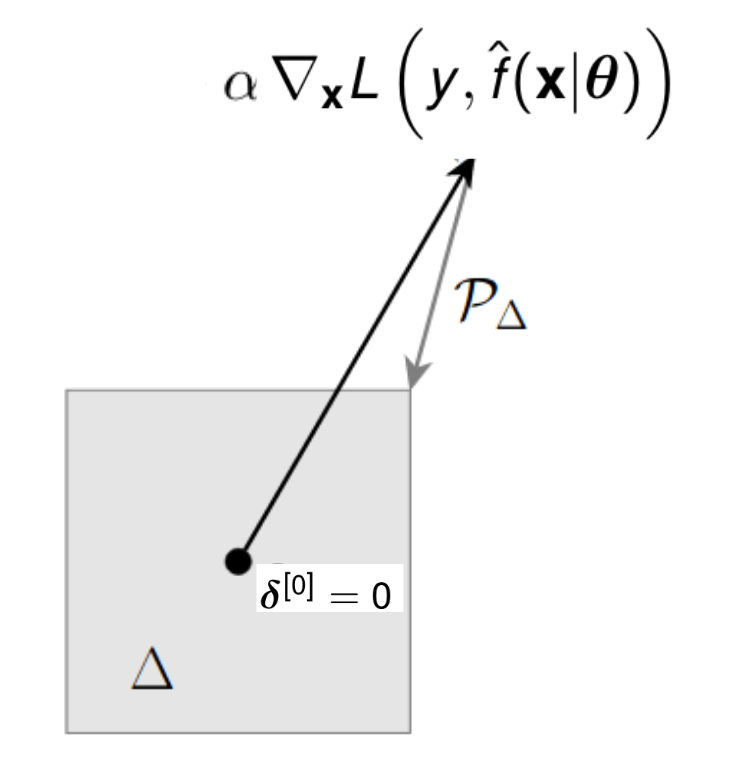
\includegraphics{plots/fgsm_mod.png}}
%       \tiny{\\Credit: Kolter and Madry}
%       \caption{$\deltab$ is obtained by setting each element of $\nabla_{\xv} L\left(y, \fh(\xv | \thetab) \right)$ to $-\epsilon$ or $\epsilon$ depending on its sign. Note that this slightly changes the direction of the step that is taken.}
%   \end{figure}
%         \item Implicitly, the (element-wise) $sign$ function is simply a way to constrain the size of the "step" that we take in the direction of the gradient. It is basically equal to a projection of the step back on $\Delta$ (which is $\mathcal{B}^{\infty}_{\epsilon}$).
%         \end{itemize}
%       \framebreak
%         \begin{itemize}
%            \item Note: The optimal attack against the linear binary classifier we saw in the last section was also FGSM!
%         %\item FGSM assumes that the linear approximation of the function given by its gradient at the point $\xv$ is a reasonably good approximation for the function over the entire region $|\deltab|_{\infty} \le \epsilon$. 
%             \end{itemize}
%   \begin{figure}
%     \centering
%       \scalebox{1}{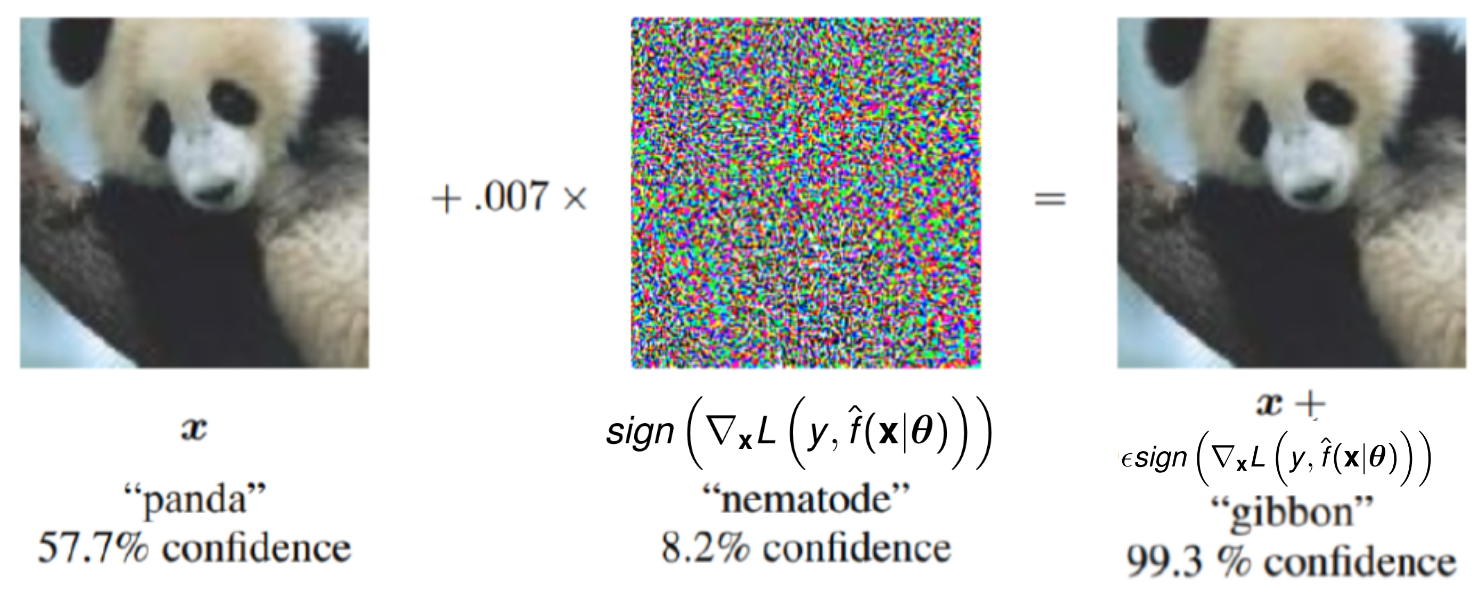
\includegraphics{plots/fgsm_panda.png}}
%       \tiny{\\Credit: Goodfellow}
%       \caption{\small{By adding an imperceptibly small vector whose elements are equal to the sign of the elements of the gradient of the cost function with respect to the input, GoogLeNet's classification of the image was changed from 'panda' to 'gibbon'. In this example, the $\epsilon$ is 0.007.}}
%   \end{figure}
% \end{vbframe}
% 
% %%%%%%%%%%%%%%%%%%%%%%%%%%%%%%%%%%%
% %\section{Adversarial Examples : A closer look (Optional)}
% %%%%%%%%%%%%%%%%%%%%%%%%%%%%%%%%%%%
% 
% %\begin{vbframe} {Adversarial Examples and Linearity}
% %  \begin{itemize}
% %    \item Goodfellow et al. (2014) showed that linear behaviour of models in high dimensional spaces is the reason for the presence of such adversarial examples.
% %    \item Neural networks are built from "mostly" linear building blocks. In the case of ReLU activations, the mapping from the input image to the output logits (the inputs to the softmax) is a piece-wise linear function.
% %    \item The value of a linear function changes rapidly if it has many inputs. Specifically, if each input is modified by $\epsilon$, a linear function with weights $\mathbf{w}$ can change by as much as $\epsilon \lVert \mathbf{w} \rVert_1$, which can be very large if $\mathbf{w}$ is high-dimensional.
% %    \item There is a tradeoff between using models that are easy to train due to their linearity and models that can use non-linear effects to become robust to adversarial perturbations. 
% %  \end{itemize}
% %\end{vbframe}
% %
% %\begin{frame} {Adversarial Examples and Linearity}
% %  \begin{figure}
% %    \centering
% %      \scalebox{0.9}{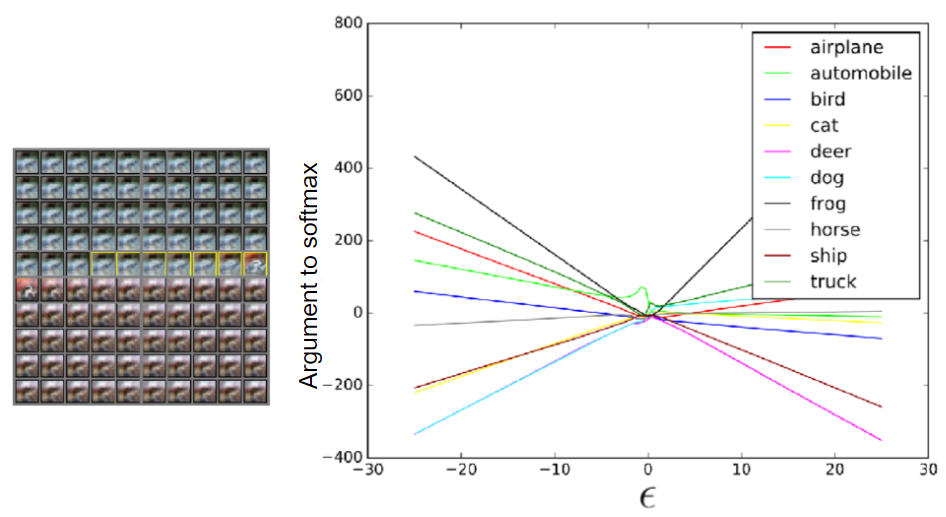
\includegraphics{plots/linear_logit.png}}
% %      \tiny{\\Credit: Goodfellow}
% %  \end{figure}
% %  \footnotesize{The figure shows the result of moving along a single direction (not necessarily axis-aligned) in the input space of a CNN. We begin with an image of an automobile (somewhere in the end of the fifth row) and move an $\epsilon$ amount in this direction (negative $\epsilon$ = opposite direction.). The images in the top half are the result of moving in the "negative $\epsilon$" direction and those in the bottom half are the result of moving in the "positive $\epsilon$" direction.}
% %\end{frame}
% %
% %\begin{frame} {Adversarial Examples and Linearity}
% %  \begin{figure}
% %    \centering
% %      \scalebox{0.9}{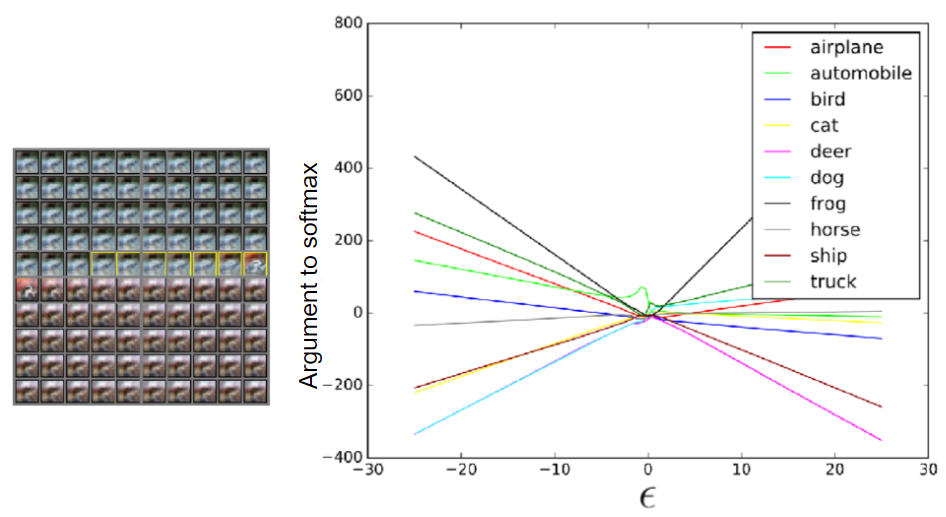
\includegraphics{plots/linear_logit.png}}
% %      \tiny{\\Credit: Goodfellow}
% %  \end{figure}
% %  \footnotesize{The figure on the right shows the logits (the inputs to the softmax) for each value of $\epsilon$. Each curve is a logit for a specific class. As we move away from the image of the automobile in either direction, the logits for the 'frog' class become extremely high and the images are misclassified by the CNN. The logits for the 'automobile' class are (relatively) high only in the middle of the plot and the CNN correctly classifies these images (yellow boxes on the left).}
% %\end{frame}
% %
% %
% %\begin{frame} {Adversarial Subspaces}
% %  \begin{figure}
% %    \center
% %      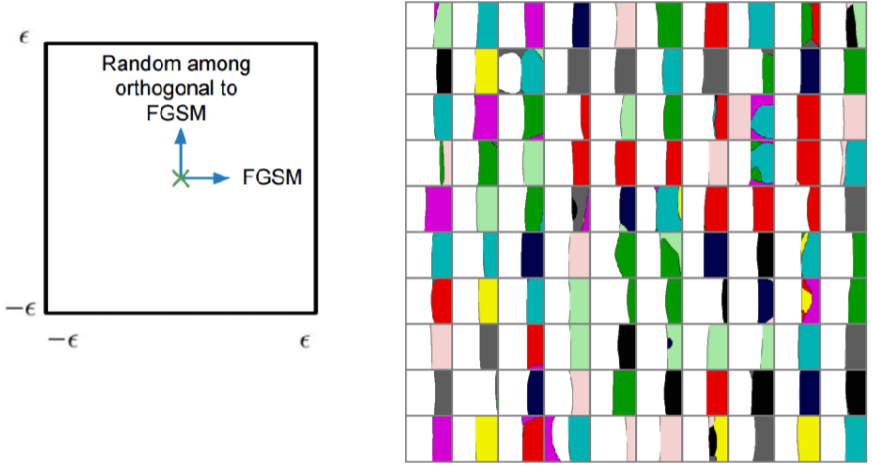
\includegraphics[width = 6.5cm]{plots/adv_cross.png}
% %      \tiny{\\Credit: Goodfellow\vspace{0.5cm}}
% %  \end{figure}
% %  \only<1>{\footnotesize Each square above represents a 2-dimensional cross section of the input space where the center corresponds to a test example (different squares = different test examples). Moving up or down in a given square indicates moving in a random direction that is orthogonal to the direction of the FGSM. White pixels indicate that the classifier outputs the correct label for the corresponding points and the colored pixels indicate that the classifier misclassifies the corresponding points (different colours = different incorrect classes).}
% %  \only<2>{The FGSM method identifies a direction such that moving along \textit{any} direction whose unit vector has a large (positive) dot product with the "FGSM vector" results in an adversarial example. Therefore, adversarial examples live in \textbf{linear subspaces} of the input space.}
% %\end{frame}
% %
% %\begin{frame} {Adversarial Subspaces}
% %  \begin{figure}
% %    \centering
% %      \scalebox{1}{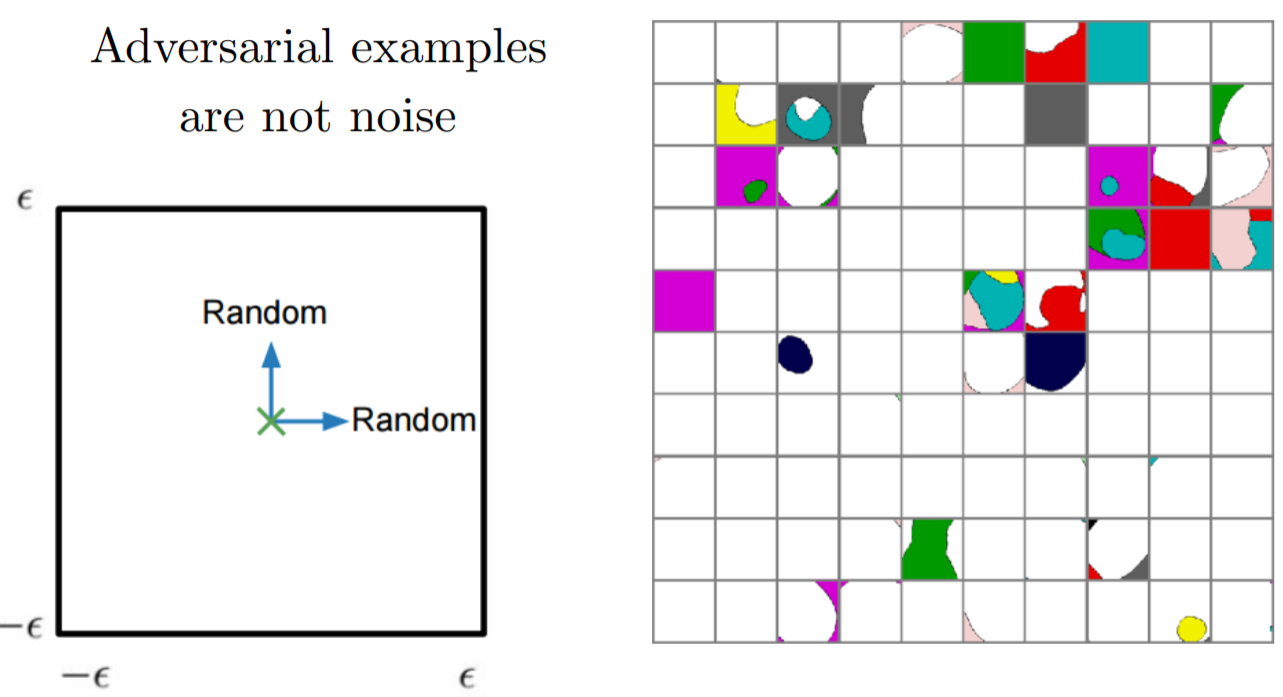
\includegraphics{plots/rand_cross.png}}
% %      \tiny{\\Credit:Goodfellow}
% %  \end{figure}
% %    For a given test example, moving in \textit{completely} random directions (within the $\epsilon$-ball) is unlikely to result in adversarial examples.
% %
% %\end{frame}
% %
% %\begin{frame} {Performance w.r.t. Uniform Distribution}
% %  \begin{figure}
% %    \centering
% %      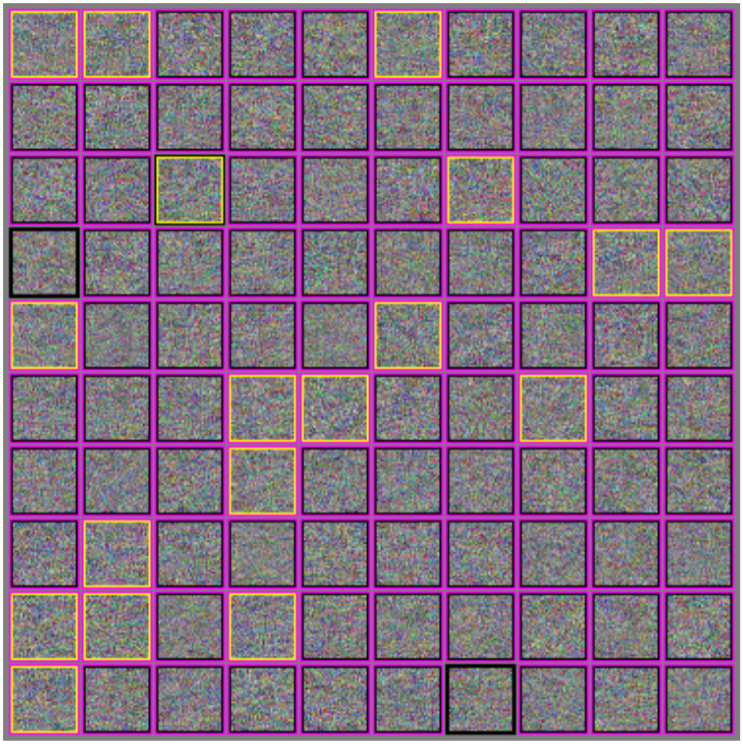
\includegraphics[width = 4cm]{plots/wrong_everywhere.png}
% %      \caption{\footnotesize Each square above corresponds to Gaussian noise that was run through a Cifar-10 classifier.}
% %  \end{figure}
% %  \small
% %      \only<1>{\small{Instead of measuring the performance of a classifier with respect to the data-generating distribution, if we measure it with respect to a uniform distribution over the whole input space, these classifiers are \textbf{wrong almost everywhere.}}}
% %      \only<2>{For all the inputs in the pink boxes, the classifier was reasonably confident (in terms of the softmax values) that the image contained something rather than nothing.}
% %      \only<3>{ For the inputs in the yellow boxes, just one step of FGSM was sufficient to convince the model that it was looking at an airplane, specifically.}
% %\end{frame}
% %
% %
% %
% %\begin{frame} {Adversarial Examples: Outlook}
% %  \begin{itemize}
% %    \item The FGSM method that we have looked at is only one of \textit{many} different algorithms for generating adversarial examples.
% %    \item Athalye et al. (2017) 3-D printed a turtle that fooled the network into classifying it as a rifle from most angles.
% %    \begin{figure}
% %    \centering
% %      \scalebox{1}{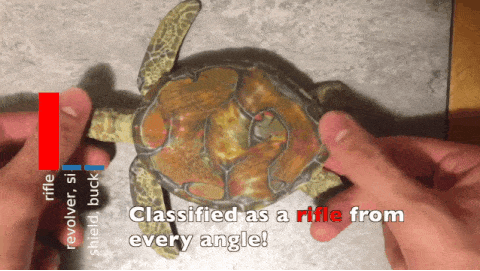
\includegraphics{plots/turtle.png}}
% %      \tiny{\\Credit: Athalye}
% %  \end{figure}
% %\end{itemize}
% %\end{frame}
% %
% %\begin{frame} {Adversarial Examples: Outlook}
% %  \begin{itemize}
% %    \item Papernot (2016) discusses ways to fool a classifier even if the model (that is, the network structure and the weights) is unknown. Such methods are called \textbf{black-box methods}.
% %    \item The library CleverHans can be used to both generate robust adversarial examples and build effective defences against adversarial attacks.
% %  \end{itemize}
% %\end{frame}
% 
% 



%%%%%%%%%%%%%%%%%%%%%%%%%%%%%%%%%%%%%%%%%%%%%%%%%%%%%%%%%%%%%%%%%%

%%%%%%%%%%%%%%%%%%%%%%%%%%%%%%%%%%%%%%%%%%%%%%%%%%%%%%%%%%%%%%%%%%
%%%%%%%%%%%%%%%%%%          REFERENCES          %%%%%%%%%%%%%%%%%%
%%%%%%%%%%%%%%%%%%%%%%%%%%%%%%%%%%%%%%%%%%%%%%%%%%%%%%%%%%%%%%%%%%
%\section{References}
\begin{vbframe}
\frametitle{References}
\footnotesize{
\begin{thebibliography}{99}
%%%%%%%%%%%%%%%%%%%%%%%%%%%%%%%%%%
\bibitem[Kolter and Madry (2019)]{1} Zico Kolter and Aleksander Madry (2019)
\newblock Adversarial Robustness - Theory and Practice
\newblock \emph{\url{https://adversarial-ml-tutorial.org/}}
%%%%%%%%%%%%%%%%%%%%%%%%%%%%%%%%%%
\bibitem[Goodfellow et al., 2016]{1} Ian Goodfellow, Yoshua Bengio and Aaron Courville (2016)
\newblock Deep Learning
\newblock \emph{\url{http://www.deeplearningbook.org/}}
%%%%%%%%%%%%%%%%%%%%%%%%%%%%%%%%%%
\bibitem[Goodfellow, 2017]{1} Ian Goodfellow (2017)
\newblock Lecture 16 | Adversarial Examples and Adversarial Training
\newblock \emph{\url{https://www.youtube.com/watch?v=CIfsB_EYsVI}}
%%%%%%%%%%%%%%%%%%%%%%%%%%%%%%%%%%
\bibitem[Goodfellow et al., 2017]{1}  Ian GoodfellowNicolas PapernotSandy HuangRocky DuanPieter AbbeelJack Clark (2017)
\newblock Attacking Machine Learning with Adversarial Examples
\newblock \emph{\url{https://openai.com/blog/adversarial-example-research/}}
%%%%%%%%%%%%%%%%%%%%%%%%%%%%%%%%%%
% \bibitem[Hastie et al., 2009]{2} Trevoe Hastie, Robert Tibshirani and Jerome Friedman (2009)
% \newblock The Elements of Statistical Learning
% \newblock \emph{\url{https://statweb.stanford.edu/\%7Etibs/ElemStatLearn/}}
% %%%%%%%%%%%%%%%%%%%%%%%%%%%%%%%%%%
\bibitem[Nguyen et al., 2015]{1} Anh Nguyen, Jason Yosinski and Jeff Clune (2015)
\newblock Deep Neural Networks are Easily Fooled: High Confidence Predictions for Unrecognizable Images
\newblock \emph{\url{https://arxiv.org/abs/1412.1897}}
%%%%%%%%%%%%%%%%%%%%%%%%%%%%%%%%%%
\bibitem[Krizhevsky et al., 2012]{1} Alex Krizhevsky, Ilya Sutskever and Geoffrey E. Hinto (2012)
\newblock ImageNet Classification with Deep Convolutional Neural Networks. NIPS. 
\newblock \emph{\url{https://papers.nips.cc/paper/4824-imagenet-classification-with-deep-convolutional-neural-networks}}
%%%%%%%%%%%%%%%%%%%%%%%%%%%%%%%%%%
% \bibitem[Hinton et al., 2012]{3} Geoffrey E Hinton, Nitish Srivastava, Alex Krizhevsky Ilya Sutskever and Ruslan Salakhutdinov (2012)
% \newblock Improving neural networks by preventing co-adaptation of feature detectors
% \newblock \emph{\url{http://arxiv.org/abs/1207.0580}}
% %%%%%%%%%%%%%%%%%%%%%%%%%%%%%%%%%%
\bibitem[Maxence Prevost (2018)]{1} Maxence Prevost (2018)
\newblock Adversarial ResNet50 
\newblock \emph{\url{http://arxiv.org/abs/1207.0580}}
%%%%%%%%%%%%%%%%%%%%%%%%%%%%%%%%%%
\bibitem[Sharif et al. (2016)]{1} Mahmood Sharif, Sruti  Bhagavatula and Lujo Bauer (2016)
\newblock Accessorize to a Crime: Real and Stealthy Attacks onState-of-the-Art Face Recognition. Proceedings of the 2016 ACM SIGSAC Conference on Computer and Communications Security.
\newblock \emph{\url{https://dl.acm.org/doi/10.1145/2976749.2978392}}
%%%%%%%%%%%%%%%%%%%%%%%%%%%%%%%%%%
\bibitem[Goodfellow et al., 2014]{5} Goodfellow, Shlens (2014)
\newblock Explaining and Harnessing Adversarial Examples
\newblock \emph{\url{https://github.com/maxpv/maxpv.github.io/blob/master/notebooks/Adversarial_ResNet50.ipynb}}
%%%%%%%%%%%%%%%%%%%%%%%%%%%%%%%%%%
\bibitem[Papernot et al., 2016]{5} Papernot , McDaniel, Goodfellow, Jha, Celik, Swamy (2016)
\newblock Practical Black-Box Attacks against Machine Learning
\newblock \emph{\url{https://arxiv.org/abs/1602.02697}}
%%%%%%%%%%%%%%%%%%%%%%%%%%%%%%%%%%
\bibitem[Athalye et al., 2017]{5} Athalye , Engstrom, Ilyas, Kwok (2017)
\newblock Synthesizing Robust Adversarial Examples
\newblock \emph{\url{https://arxiv.org/abs/1707.07397}}
%%%%%%%%%%%%%%%%%%%%%%%%%%%%%%%%%%
\bibitem[Brown et al., 2018]{1} Tom B. Brown and Catherine Olsson, Research Engineers, Google Brain Team (2018)
\newblock 
Introducing the Unrestricted Adversarial Examples Challenge 
\newblock \emph{\url{https://ai.googleblog.com/2018/09/introducing-unrestricted-adversarial.html}}
%%%%%%%%%%%%%%%%%%%%%%%%%%%%%%%%%%
\end{thebibliography}
}
\end{vbframe}
%%%%%%%%%%%%%%%%%%%%%%%%%%%%%%%%%%%%%%%%%%%%%%%%%%%%%%%%%%%%%%%%%%
%%%%%%%%%%%%%%%%%%%%%%%%%%%%%%%%%%%%%%%%%%%%%%%%%%%%%%%%%%%%%%%%%%
\endlecture
\end{document}
